\documentclass[a4paper,12pt]{article}
\usepackage[utf8]{inputenc}
\usepackage[T1]{fontenc}
\usepackage[french]{babel}
\usepackage{graphicx}
\usepackage{hyperref}
\usepackage{enumitem}
\usepackage{microtype}
\usepackage{mathpazo}      % Police élégante
\usepackage[T1]{fontenc}   % Pour une bonne gestion des accents
\microtypesetup{expansion=false}
\usepackage{float}
\usepackage[a4paper,margin=2.5cm]{geometry}
\usepackage{titlesec}
\titleformat{\section}{\Large\bfseries\sffamily}{\thesection}{1em}{}
\titleformat{\subsection}{\large\bfseries\sffamily}{\thesubsection}{1em}{}
\usepackage{fancyhdr}



\begin{document}
\begin{titlepage}
\newgeometry{margin=2.5cm}
\centering

\vspace*{4cm}
{\Huge\bfseries Guide d'Utilisation pour la prise en main de notre application d'aide a l'archivage et a la consultation des projets de fin d'année des etudiants.\par}
\vspace{0.5cm}
{\LARGE\itshape AcadProManage \par}
\vspace{2cm}
\vfill


\restoregeometry
\thispagestyle{fancy}
\end{titlepage}
\newpage

\tableofcontents
\newpage


\pagestyle{fancy} % Active le style "fancy"

% En-têtes personnalisés
\fancyhead[L]{}    % En-tête gauche : nom de la plateforme
\fancyhead[C]{}                 % En-tête centre : vide
\fancyhead[R]{}         % En-tête droite : numéro de page

% Pieds de page personnalisés
\fancyfoot[L]{AcadProManage}                 % Pied gauche : vide
\fancyfoot[C]{} % Pied centre : titre + date
\fancyfoot[R]{\thepage}                 % Pied droit : vide
\setlength{\headheight}{15pt} % ou 20pt si tu as des erreurs de hauteur
\setlength{\footskip}{30pt}

%\begin{titlepage}
%\centering
%\vspace*{2cm}
%{\Huge\bfseries Guide d'utilisation d'AcadProManage \par}
%\vspace{2cm}
%{\Large Version 2.0 \par}
%\vspace{1cm}
%{\Large Christian Nana \par}
%\vspace{3cm}
%\includegraphics[width=0.5\textwidth]{IMAGES/logo-acadpromanage.png}  facultatif
%\vfill
%{\large \today}
%\end{titlepage}



\addcontentsline{toc}{section}{Liste des figures}
\listoffigures
\vspace{2cm}
\newpage

\section*{Introduction}
\addcontentsline{toc}{section}{introduction}
Dans un contexte académique où la gestion des projets étudiants devient un enjeu crucial, la plateforme AcadProManage vise à centraliser, organiser et valoriser les travaux des apprenants. Ce guide a été conçu pour faciliter la prise en main de l’outil et optimiser l'expérience utilisateur, en particulier pour les étudiants, enseignants et encadreurs de projets.
\newpage
\section*{1. Page d'Accueil}
\addcontentsline{toc}{section}{1. page d'Accueil}
Lorsque vous arrivez sur le site, vous verrez la page d'accueil. C'est le point de départ pour toutes vos activités sur AcadProManage.

Recherche de projets : Vous pouvez rechercher des projets en entrant un mot-clé ou un nom d'auteur dans la barre de recherche située en haut de la page.

Parcourir les domaines : La page d'accueil affiche également les meilleurs domaines avec le nombre de projets associés (ex : Intelligence Artificielle, Cyber Sécurité, Block Chain, Réseau, Data Science, Génie Logiciel).

Navigation principale : En haut de la page, vous trouverez des liens pour "Accueil", "Domaines", "Projets", "Contact" et la sélection de la "Langue".

Se connecter : Pour accéder à votre espace personnel ou créer un compte, cliquez sur le bouton "Se Connecter" en haut à droite.

Voici un aperçu de la page d'accueil d'AcadProManage :

%% Position image ici : page d'accueil
\begin{figure}[H] 
\centering
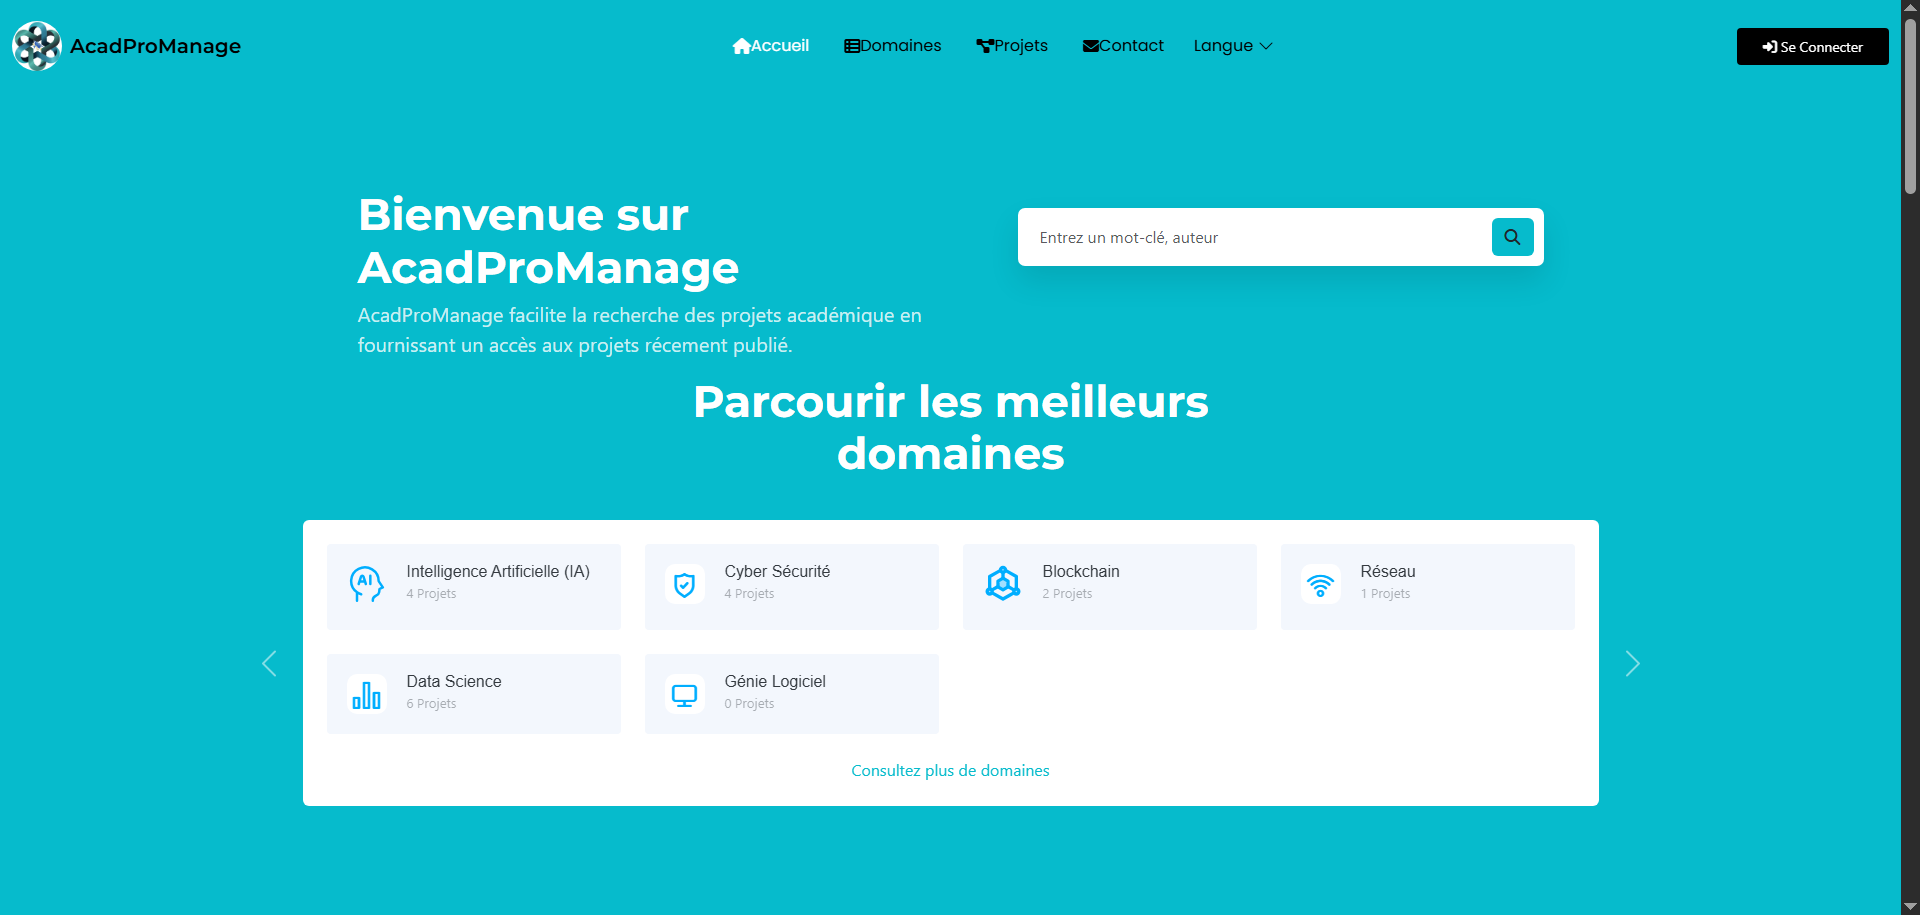
\includegraphics[width=0.9\textwidth]{IMAGES/Accueil.png}
\caption{Aperçu de la page d’accueil}
\label{fig:Accueil}
\end{figure}


\section*{2. Connexion et Création de Compte}
\addcontentsline{toc}{section}{2.Connexion et création de compte}
\subsection*{2.1. Se Connecter}
\addcontentsline{toc}{subsection}{2.1 Se Connecter }

\begin{quote}
Pour accéder à votre tableau de bord ou à d'autres fonctionnalités réservées aux utilisateurs, vous devrez vous connecter.

Cliquez sur le bouton "Se Connecter" en haut à droite de la page d'accueil.

Une fenêtre pop-up "Connectez Vous" apparaîtra.

Entrez votre adresse email dans le champ "Email".

Entrez votre mot de passe dans le champ "Mot de passe".

Cliquez sur le bouton "Se Connecter".

Si vous avez oublié votre mot de passe, cliquez sur "Mot de passe oublié ?".

Si vous n'avez pas de compte, cliquez sur "Créer un compte".

L'écran de connexion ressemble à ceci :

%% Position image ici : écran de connexion
\begin{figure}[H]
\centering
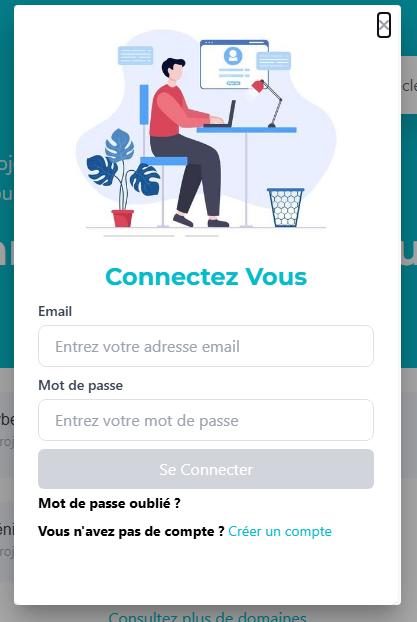
\includegraphics[width=0.9\textwidth]{IMAGES/Connexion.png}
\caption{Écran de connexion de la plateforme AcadProManage}
\label{fig:ecranconnexion}
\end{figure}



\end{quote}

\subsection*{2.2. Créer un Compte}
\addcontentsline{toc}{subsection}{2.2 Créer un Compte}
\begin{quote}
Si vous êtes un nouvel utilisateur, suivez ces étapes pour créer votre compte.

Depuis la fenêtre de connexion, cliquez sur "Créer un compte".

Une fenêtre pop-up "Créer un compte" s'affichera, vous guidant à travers deux étapes.

\underline{Étape 1 :} Informations personnelles La première étape consiste à fournir vos informations de base.

Entrez votre nom dans le champ "Nom".

Entrez votre adresse email dans le champ "Email".

Sélectionnez votre filière dans le menu déroulant "Filière".

Cliquez sur "Suivant" pour passer à l'étape 2.

Voici la présentation de l'étape 1 de la création de compte :

%% Position image ici : étape 1 création de compte
\begin{figure}[H]
\centering
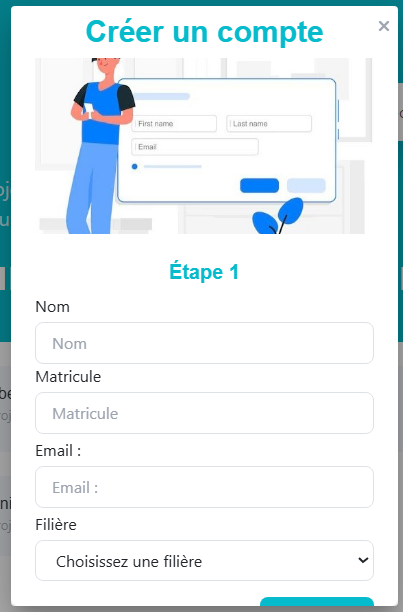
\includegraphics[width=0.85\textwidth]{IMAGES/creercompte1.png}
\caption{Présentation de l'étape 1 de la création de compte}
\label{fig:etape1}
\end{figure}

\underline{Étape 2 :} Mot de passe Après avoir rempli vos informations personnelles, vous définirez votre mot de passe.

Entrez votre mot de passe dans le champ "Mot de passe".

Confirmez votre mot de passe en le saisissant à nouveau dans le champ "Confirmer Mot de passe".

Cliquez sur "S'inscrire" pour finaliser la création de votre compte.

Vous pouvez revenir à l'étape précédente en cliquant sur "Précédent".

L'écran pour l'étape 2 de la création de compte est le suivant :

%% Position image ici : étape 2 création de compte
\begin{figure}[H]
\centering
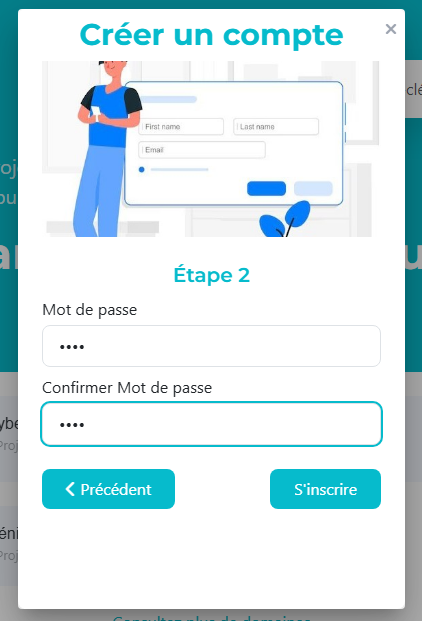
\includegraphics[width=0.85\textwidth]{images/creercompte2.png}
\caption{Écran pour l'étape 2 de la création de compte}
\label{fig:etape2}
\end{figure}
\end{quote}


\section*{3. Tableau de Bord de l'Utilisateur (Dashboard)}
\addcontentsline{toc}{section}{3. Tableau de Bord de l'Utilisateur (Dashboard)}
\begin{quote}
Une fois connecté, vous accéderez à votre tableau de bord personnel. C'est ici que vous gérerez vos projets et vos informations de profil.

Bienvenue : Vous serez accueilli avec le message "Bienvenue dans votre espace personnel".

Navigation du tableau de bord : Sur le côté gauche, vous trouverez un menu de navigation :

JEAN JACK Dashboard (votre nom d'utilisateur)

PAGES :
My Projects
Profile
Settings

Rechercher un projet : Une barre de recherche est disponible pour rechercher vos projets.

Visualiser vos projets : Vos projets seront affichés sous forme de cartes, indiquant leur statut (Approuvé, Rejeté) et la date de publication.

Voici un exemple de tableau de bord utilisateur :

%% Position image ici : tableau de bord
\begin{figure}[H]
\centering
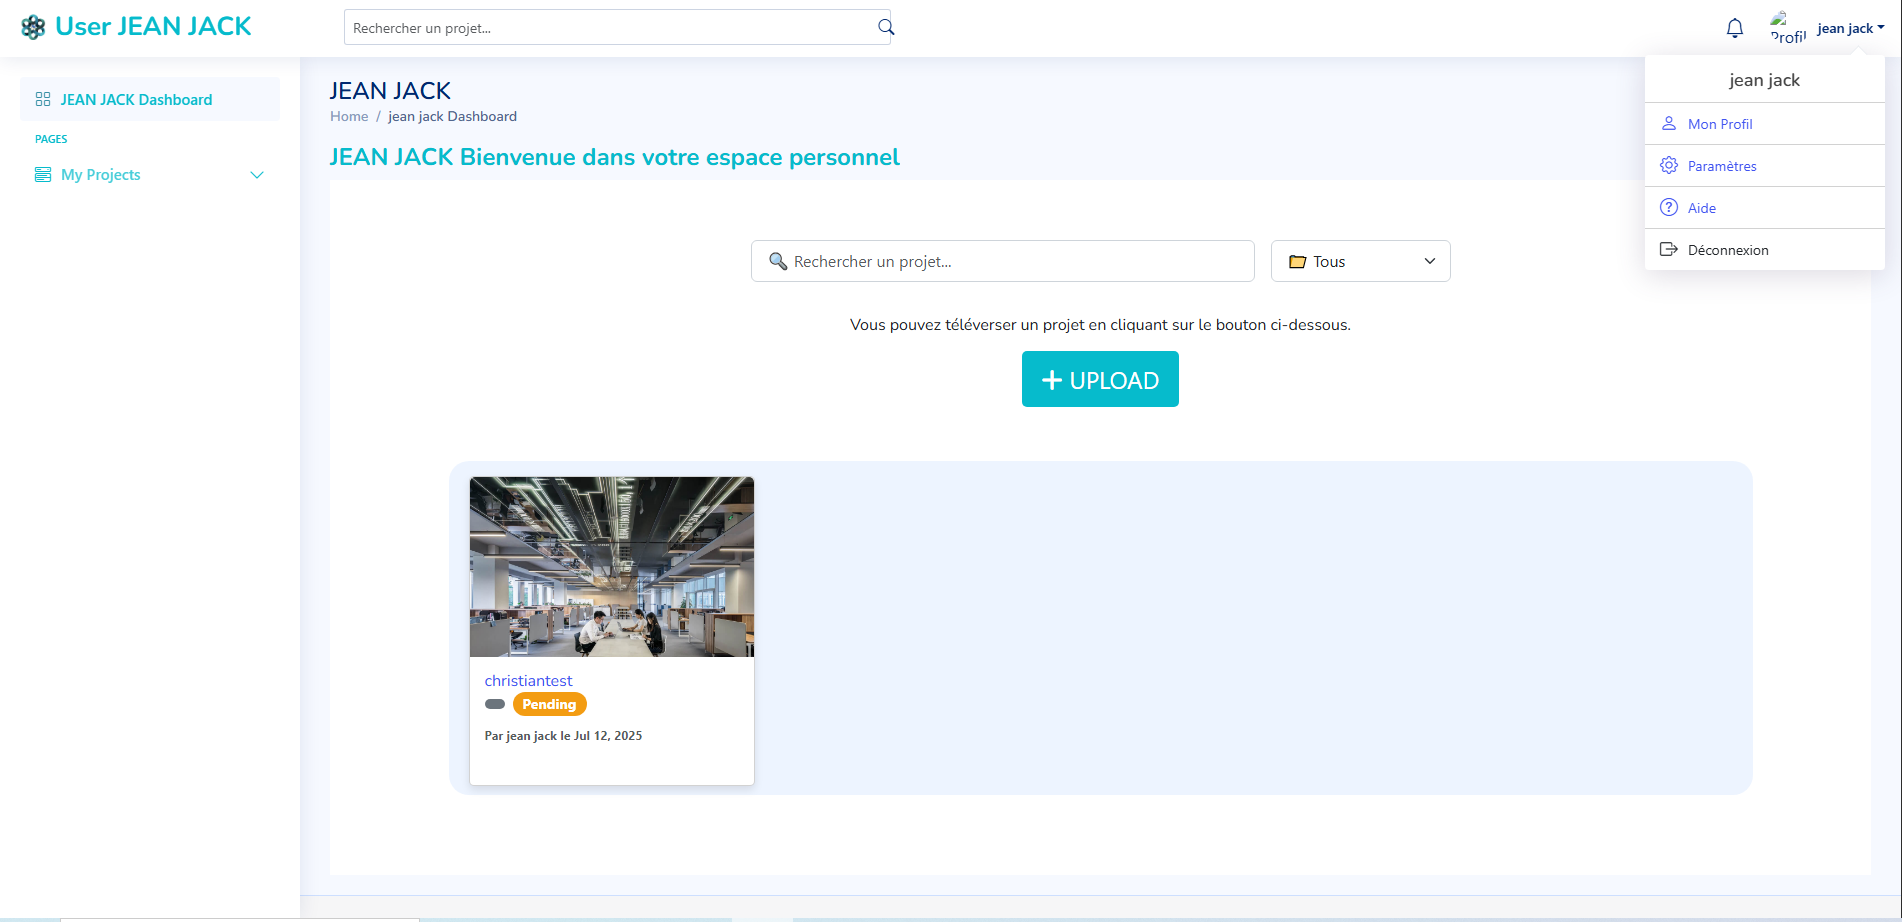
\includegraphics[width=0.9\textwidth]{IMAGES/dashboard-utilisateur.png}
\caption{Exemple de tableau de bord utilisateur}
\label{fig:dashboard}
\end{figure}

\end{quote}
\section*{4. Créer un Projet (Upload d'un Document)}
\addcontentsline{toc}{section}{4. Créer un Projet (Upload d'un Document)}
\begin{quote}
Depuis votre tableau de bord, vous avez la possibilité d’ajouter un nouveau projet. Ce processus se déroule en plusieurs étapes.

Cliquez sur le bouton "+ UPLOAD" pour commencer le processus de création de projet.

Une fenêtre pop-up "Créer un projet" apparaîtra, vous guidant à travers six étapes.

\underline{Step 1 :} Project Info La première étape concerne les informations de base de votre projet.

Entrez le titre de votre projet dans le champ "Titre".

Sélectionnez le type de projet dans le menu déroulant "Type Projet".

Pour "Couverture du Projet", cliquez sur "Choisir un fichier" pour télécharger un fichier de couverture pour votre projet.

Cliquez sur "Next" pour passer à l'étape suivante.

%% Voici la fenêtre pour l'étape 1 de la création de projet :

%% Position image ici : étape 1 création projet
\begin{figure}[H]
\centering
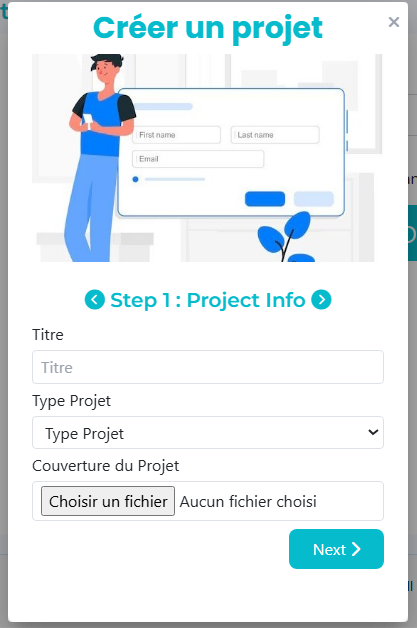
\includegraphics[width=0.85\textwidth]{IMAGES/etape1-projet.png}
\caption{Fenêtre pour l'étape 1 de la création de projet}
\label{fig:etape1projet}
\end{figure}
\underline{Step 2 :} Project Info La deuxième étape vous demande de préciser votre niveau d’étude et la catégorie de votre projet.

Sélectionnez le niveau de votre projet dans le menu déroulant "Niveau".

Sélectionnez la catégorie de votre projet dans le menu déroulant "Catégorie".

Cliquez sur "Next" pour continuer.

Cliquez sur "Previous" pour revenir à l'étape précédente.

Voici la fenêtre pour l'étape 2 de la création de projet :

%% Position image ici : étape 2 création projet
\begin{figure}[H]
\centering
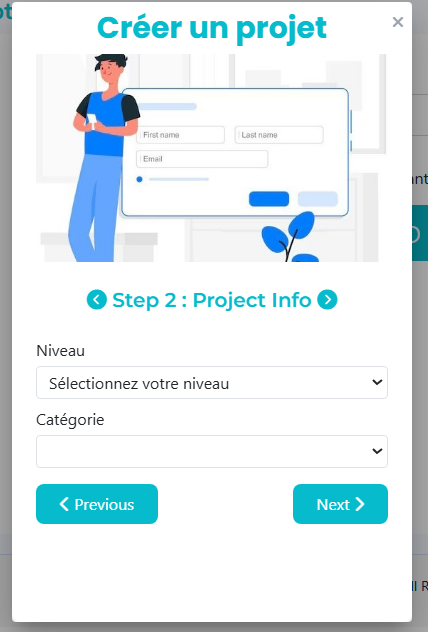
\includegraphics[width=0.85\textwidth]{IMAGES/etape2-projet.png}
\caption{Fenêtre pour l'étape 2 de la création de projet}
\label{fig:etape2projet}
\end{figure}

\underline{Step 3 :} Project Info cette étape consiste à fournir un résumé de votre projet.

Entrez une description ou un résumé de votre projet dans le champ "Resume".

Cliquez sur "Next" pour continuer.

Cliquez sur "Previous" pour revenir à l'étape précédente.

Voici la fenêtre pour l'étape 3 de la création de projet :

%% Position image ici : étape 3 création projet
\begin{figure}[H]
\centering
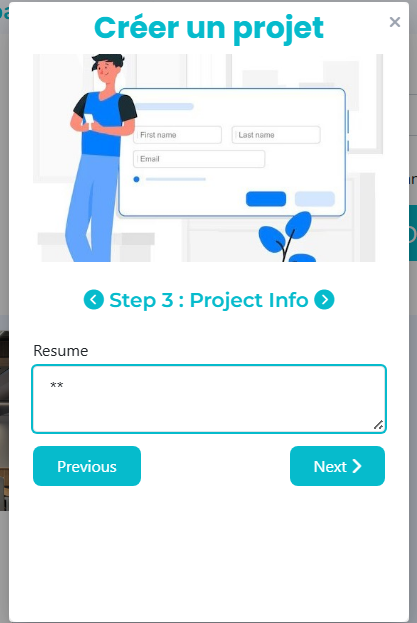
\includegraphics[width=0.85\textwidth]{IMAGES/etape3-projet.png}
\caption{Fenêtre pour l'étape 3 de la création de projet}
\label{fig:etape3projet}
\end{figure}

\underline{Step 4 :} Document Info Ajoutez les documents pertinents pour votre projet.

Entrez le nom du document dans le champ "Nom du document".

Choisissez le fichier de votre document en cliquant sur "Choisir un fichier”. Puis Cliquer sur "+ Add"

Cliquez sur "+ Add" pour ajouter d'autres documents si votre projet en contient plusieurs, ou "Next" pour passer à étape suivante.


%% Position image ici : étape 4 création projet
\begin{figure}[H]
\centering
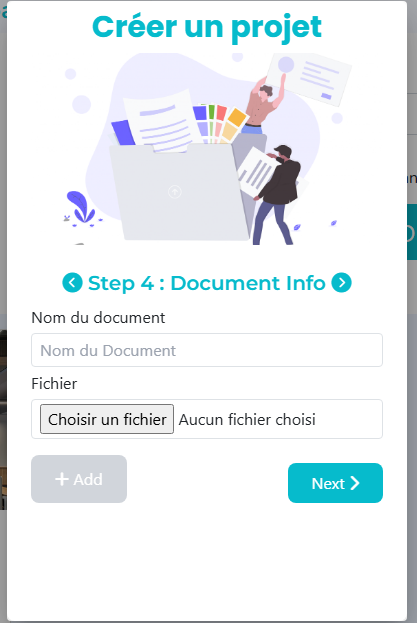
\includegraphics[width=0.85\textwidth]{IMAGES/etape4-projet.png}
\caption{Fenêtre pour l'étape 4 de la création de projet}
\label{fig:etape4projet}
\end{figure}

\underline{Step 5 :} Collaborators ici vous Indiquez les collaborateurs qui ont contribué à votre projet.

Entrez le nom du collaborateur dans le champ "Nom du Collaborateur".

Entrez l'adresse email du collaborateur dans le champ "Email du Collaborateur". Puis Cliquer sur "+ Add"

Cliquez sur "+ Add" pour ajouter d'autres collaborateurs, ou "Next" pour passer aux informations du superviseur. Notez que les champs marqués d'un point d'exclamation rouge (par exemple, "Nom du collaborateur requis !", "Adresse Email requis !") sont requis.

(NB : cette étape n’est pas obligatoire dans la mesure ou vous êtes seul à travailler sur votre rapport)

Voici la fenêtre pour l'étape 4 de la création de projet :

%% Position image ici : étape 5 création projet
\begin{figure}[H]
\centering
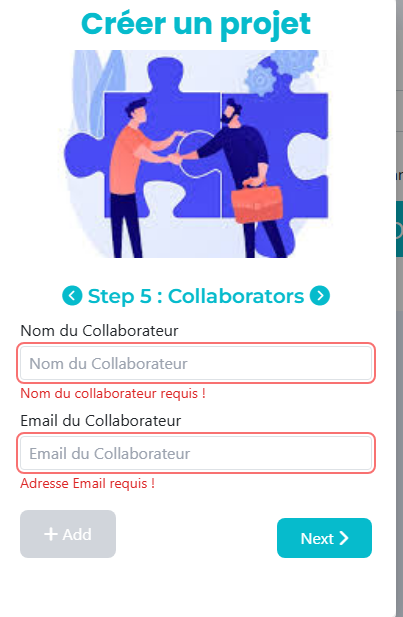
\includegraphics[width=0.85\textwidth]{IMAGES/etape5-projet.png}
\caption{Fenêtre pour l'étape 5 de la création de projet}
\label{fig:etape5projet}
\end{figure}

\underline{Step 6 :} Supervisor Info Vous Finalisez la création de votre projet en ajoutant les informations de votre superviseur.

Entrez le nom du superviseur dans le champ "Nom du Superviseur".

Entrez l'adresse email du superviseur dans le champ "Email du Superviseur".

Cliquez sur "+ Add" pour ajouter d'autres superviseurs si nécessaire, ou "Finish" pour compléter et soumettre votre projet. Les champs requis sont signalés par un point d'exclamation rouge.

Voici la fenêtre pour l'étape 6 de la création de projet :

%% Position image ici : étape 6 création projet
\begin{figure}[H]
\centering
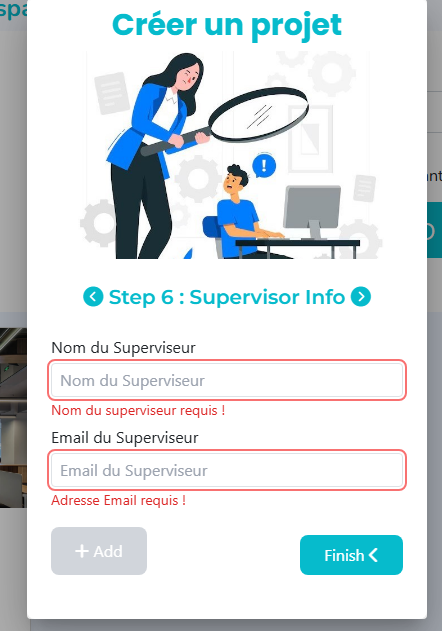
\includegraphics[width=0.85\textwidth]{IMAGES/etape6-projet.png}
\caption{Fenêtre pour l'étape 6 de la création de projet}
\label{fig:etape6projet}
\end{figure}
\end{quote}

\section*{4.1 Gérer les documents du projet}
\addcontentsline{toc}{section}{4.1 Gérer les documents du projet}
\begin{quote}
Une fois un projet créé, vous avez la possibilité de gérer votre projet, visualiser la liste des collaborateurs déjà associés à votre projet sous la section "Collaborators Related".

Dans la page de détails de votre projet (accessible en faisant un double clic sur votre projet crée) :

Cliquez sur "Add Document" pour ajouter de nouveaux fichiers pertinents à votre projet.

Cliquez sur "Add Supervisor" pour associer des superviseurs à votre travail.

Cliquez sur "Add Collaborator" pour inviter de nouvelles personnes à contribuer.

Cliquez sur "Delete" pour supprimer votre projet.

Voici un aperçu de la page de détails d’un projet :

%% Position image ici : détails du projet
\begin{figure}[H]
\centering
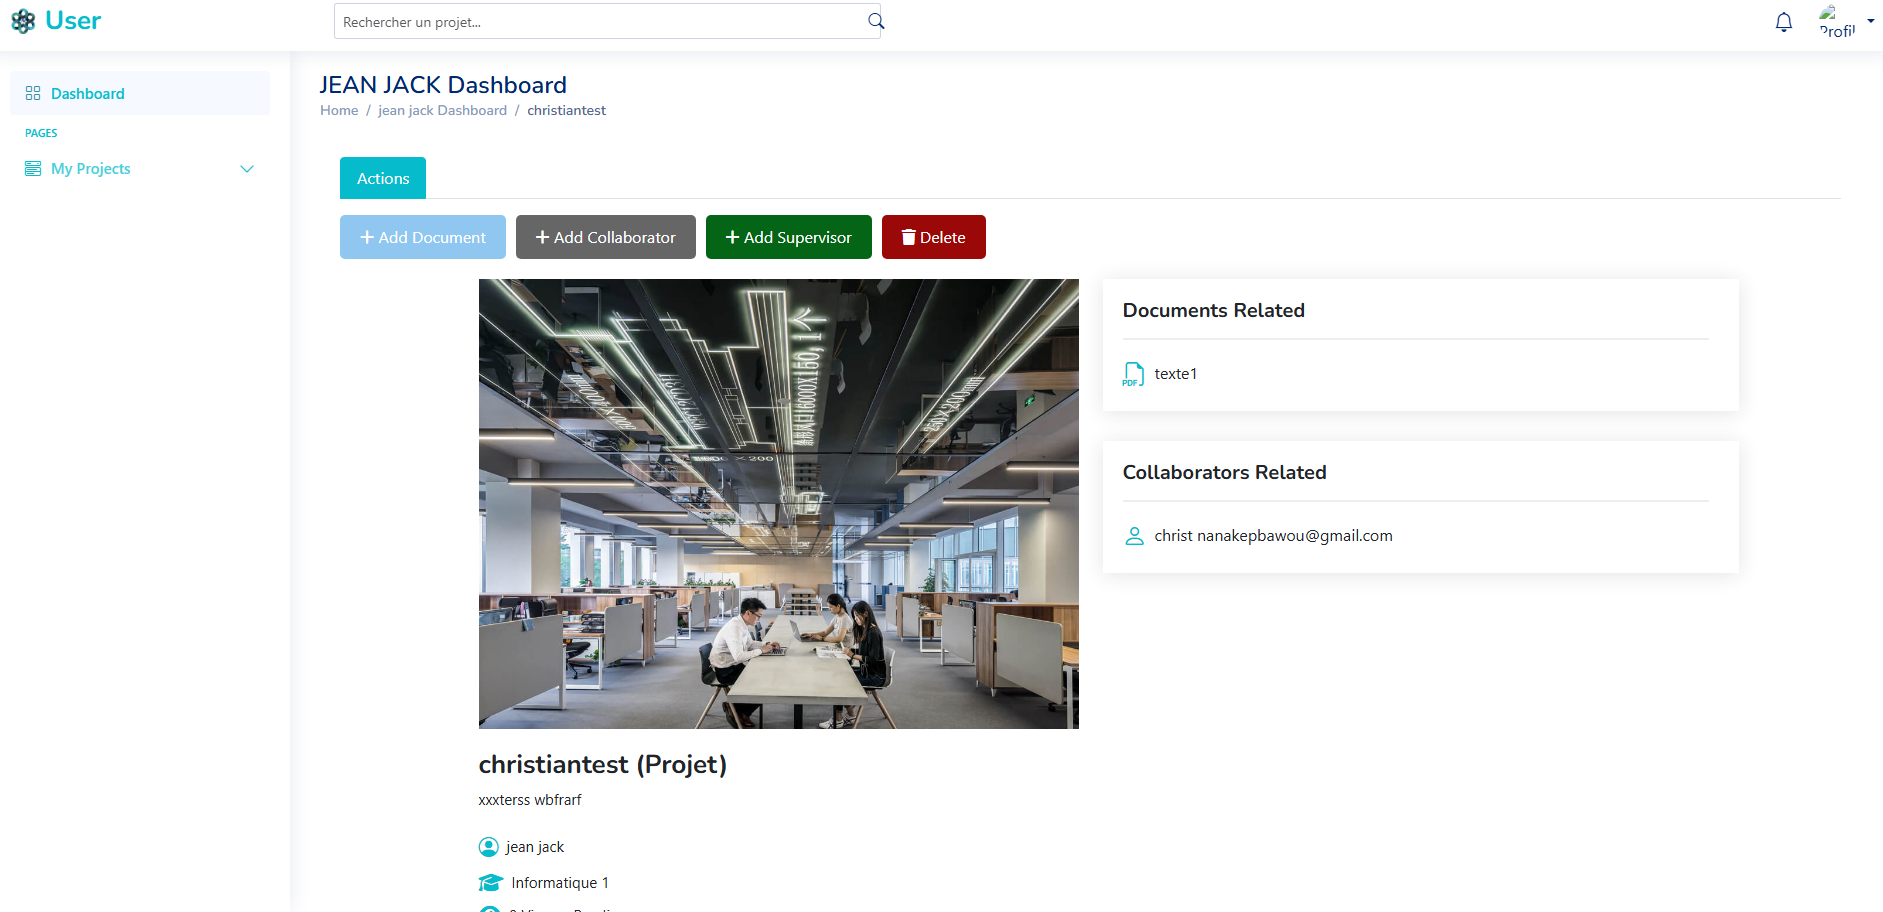
\includegraphics[width=0.85\textwidth]{IMAGES/details-projet.png}
\caption{Aperçu de la page de détails d’un projet}
\label{fig:detailprojet}
\end{figure}

\end{quote}

\section*{5. Gestion du Profil}
\addcontentsline{toc}{section}{5. Gestion du Profil}
\begin{quote}
Vous pouvez gérer les informations de votre profil depuis votre tableau de bord. Cela vous permet de maintenir vos coordonnées à jour.
\end{quote}
\subsection*{5.1. Accéder au Profil}
\addcontentsline{toc}{subsection}{5.1. Accéder au Profil}
\begin{quote}
Pour accéder à votre profil Cliquez "Mon Profil" depuis le menu déroulant en haut à droite (sous votre nom d'utilisateur).

Dans votre page de profil :

Modifier Nom/Prénom : Cliquez sur "Modifier Nom/Prénom" pour changer votre nom et prénom. Entrez le nouveau "Nom" et "Prénom" et cliquez sur "Enregistrer".

Modifier Email : Cliquez sur "Modifier Email" pour changer votre adresse email.

Modifier Mot de passe : Cliquez sur "Modifier Mot de passe" pour changer votre mot de passe.

Modifier Photo : Cliquez sur "Modifier Photo" pour changer votre photo de profil.

Voici à quoi ressemble l'interface pour modifier votre profil :

%% Position image ici : modification du profil
\begin{figure}[H]
\centering
\includegraphics[width=0.85\textwidth]{IMAGES/modification-profil.png}
\caption{Interface pour modifier votre profil}
\label{fig:modifprofil}
\end{figure}

\end{quote}

\section*{6. Déconnexion}
\addcontentsline{toc}{section}{6. Déconnexion}
\begin{quote}
Pour vous déconnecter de votre compte et sécuriser votre session, suivez cette simple étape.

Cliquez sur votre nom d'utilisateur en haut à droite, puis sélectionnez "Déconnexion" dans le menu déroulant.
\end{quote}

\begin{quote}
\newpage
\section*{Conclusion}
\addcontentsline{toc}{section}{Conclusion}

Vous voilà arrivé à la fin de ce guide d’utilisation. Nous espérons qu’il vous a permis de prendre en main les fonctionnalités essentielles d’AcadProManage avec clarté et efficacité.

Pour aller plus loin ou en cas de question, la page d’aide (Aide) est là pour vous accompagner. Accédez-y à tout moment via le menu déroulant situé en haut à droite de de votre tableau de bord. Elle regroupe :

Des réponses aux questions fréquentes (FAQ),

Des tutoriels illustrés,

Des contacts pour échanger directement avec notre équipe

Votre expérience utilisateur est notre priorité : n’hésitez pas à consulter l’aide dès que nécessaire. Merci pour votre confiance et bonne utilisation !
\end{quote}
\end{document}
